\begin{folhaderosto}
Master's thesis, presented to the University Center of FEI for the purpose of obtaining the degree of Master of Scince (MS.c) in Electrical Engineering. Main advisor Prof. Dr. Plinio Thomaz Aquino Junior.
\end{folhaderosto}

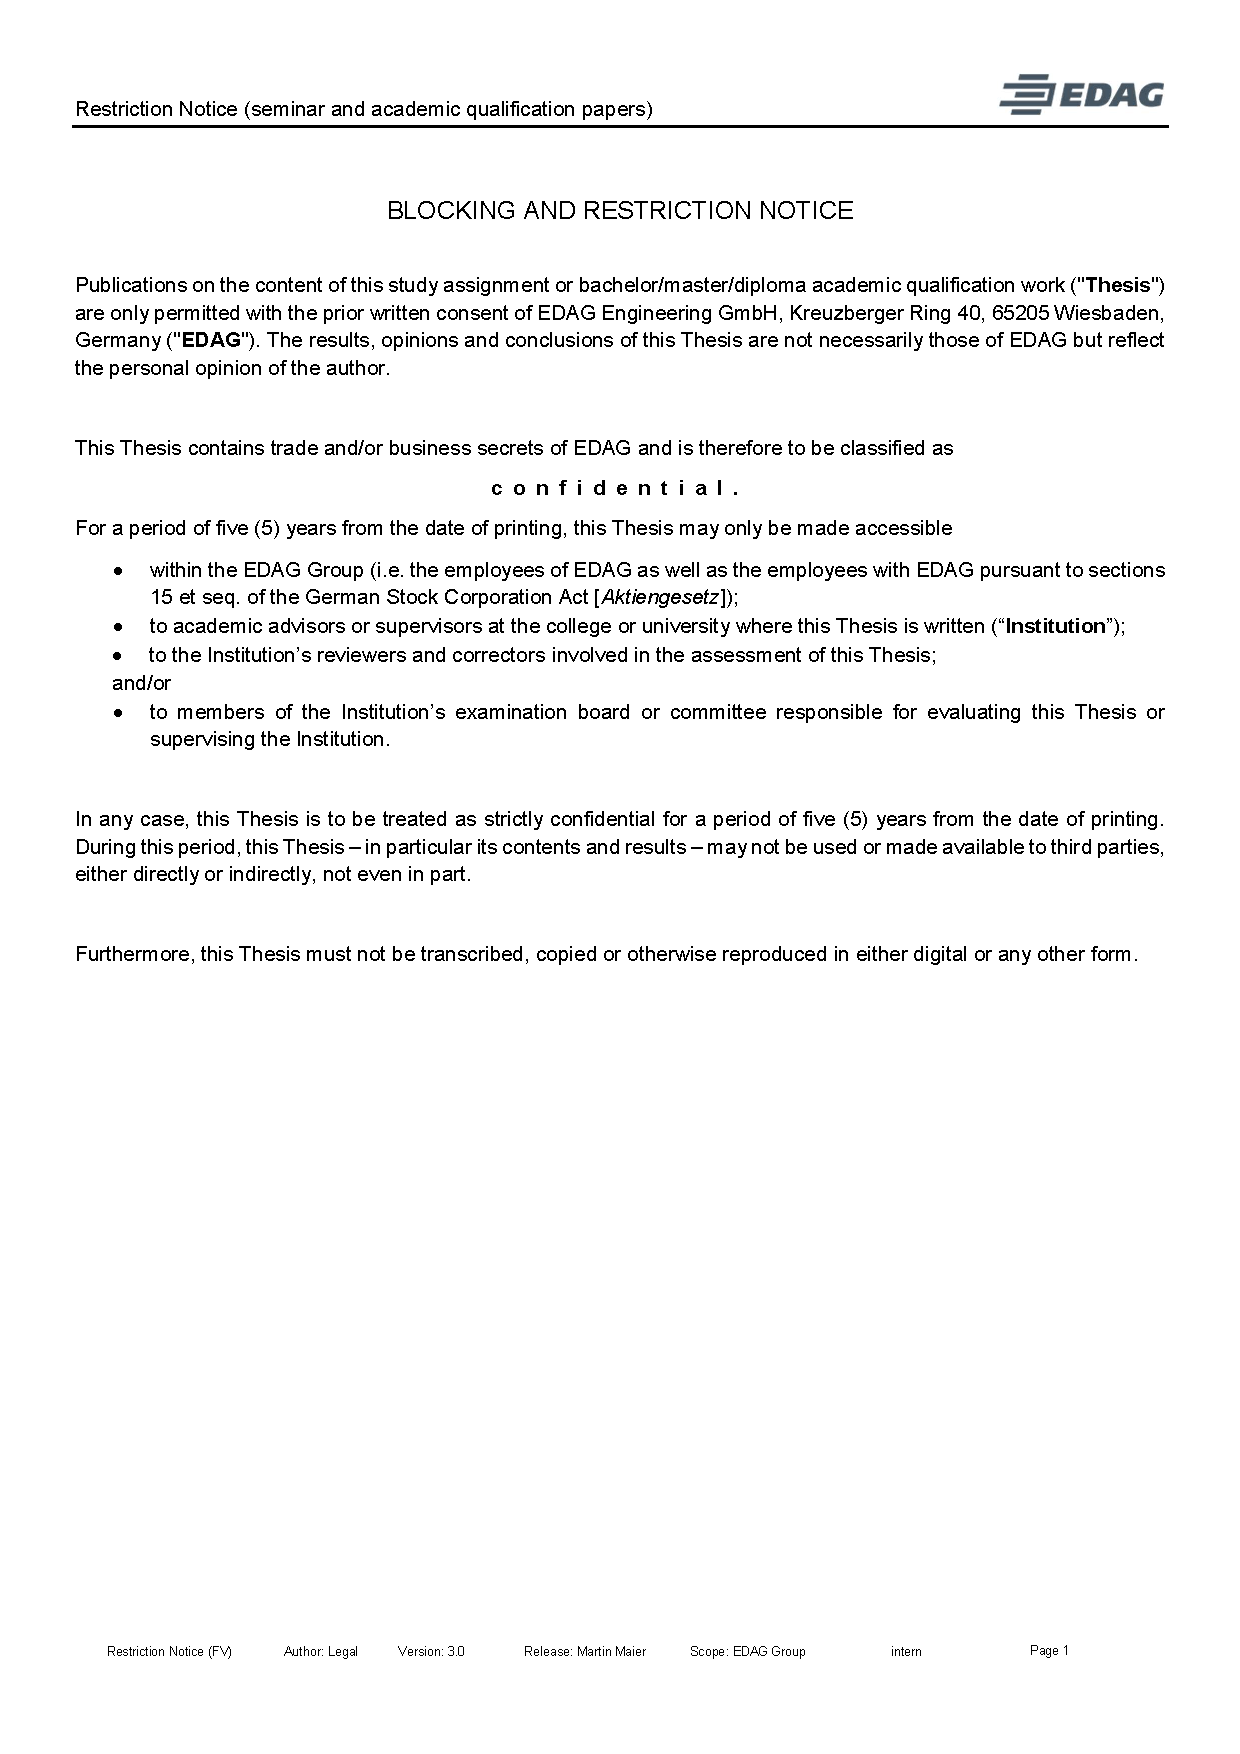
\includepdf{_blocking_notice.pdf}

\fichacatalografica
\folhadeaprovacao

% Quando disponível, substituir as duas linhas acima pelos PDFs carregados no documento.
%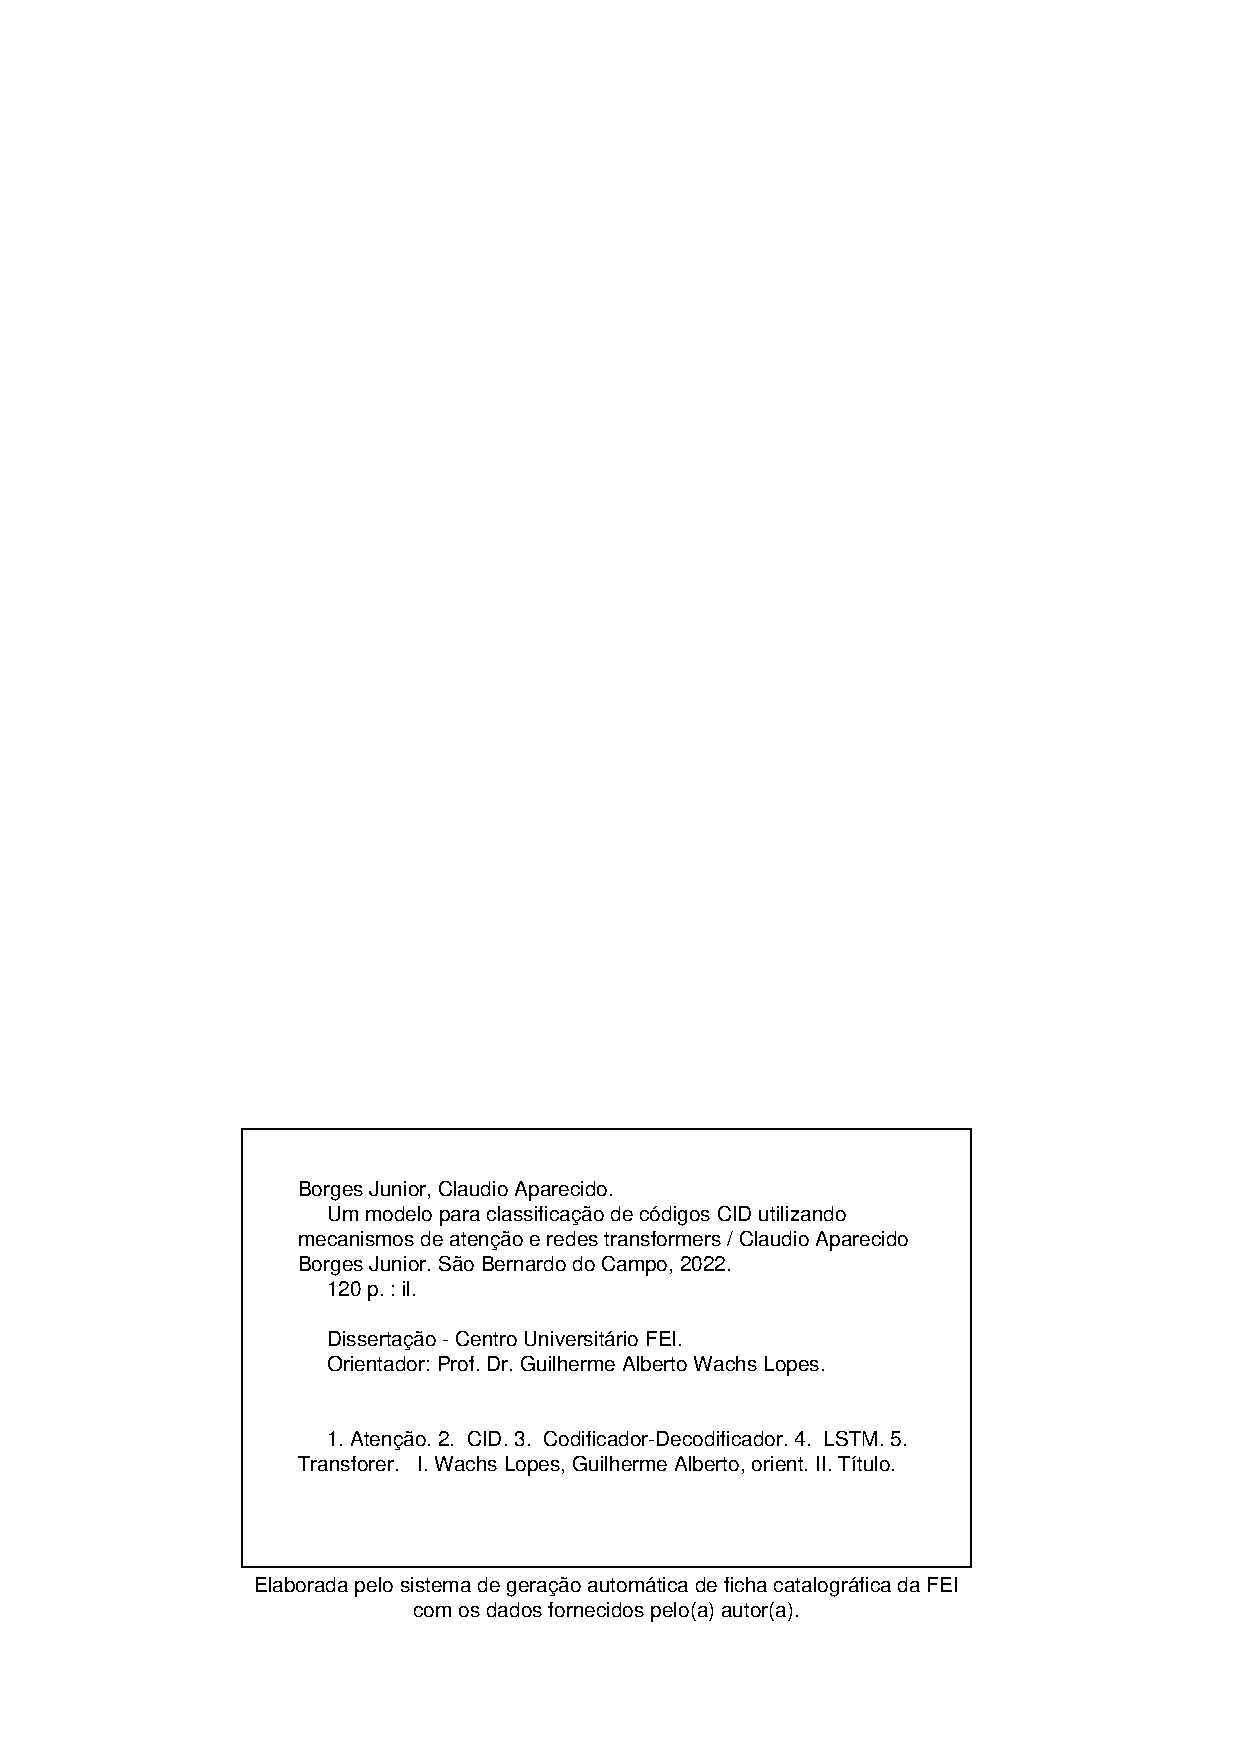
\includepdf{_ficha_catalografica.pdf}

\dedicatoria{I dedicate this study to Almighty God, to my beloved wife Priscila, and in loving memory of my parents who guided me along the path of integrity, choosing what is right over what is easy.}

\begin{agradecimentos}
First and foremost, I would like to express my profound gratitude to God for the gift of life and the resilience provided to navigate challenges.

My heartfelt thanks go to my advisor, Prof. Dr. Plinio Thomaz Aquino Junior, for unwavering support throughout all stages of this study. I am also grateful to my former advisor, Prof. Dr. Guilherme Alberto Wachs Lopes, whose guidance introduced me to essential tools for the completion of this dissertation.

I extend my appreciation to the entire staff at FEI and my work colleagues at EDAG GmbH. Special thanks to Mr. Martin Vollmer and Mr. Alexandre Sberveglieri for their invaluable contributions to my professional development, and to Mr. Johannes Barckmann, Mr. Michael Jahn, and Mr. Maximilan Happel for their support in this project.

Finally, I am deeply indebted to my beloved wife, whose unconditional support served as a constant source of strength during these three years. In moments of discouragement, her presence was my sanctuary, providing me hope and inspiration to continue moving forward.
\end{agradecimentos}

\begin{epigrafe}
	\epig{Our greatest weakness lies in giving up. The most certain way to succeed is always to try just one more time.}{Thomas A. Edison}
	\epig{We don't have better algorithms, we just have more data.}{Peter Norvig}
\end{epigrafe}